\documentclass{beamer}
\usepackage{hyperref}
\usepackage{amsmath}
\usepackage{multirow}
\usepackage{wrapfig}
\usepackage{alltt}
\usepackage{float}
\usepackage{subfig}
\usepackage{multirow}
\usepackage{tabularx}


\usetheme{beaver}
\setbeamertemplate{footline}[frame number]{}
\setbeamertemplate{navigation symbols}{}

\AtBeginSection{\frame{\sectionpage}}
\AtBeginSubsection{\frame{\subsectionpage}}

\defbeamertemplate{section page}{mine}[1][]{%
  \begin{centering}
    {\usebeamerfont{section name}\usebeamercolor[fg]{section name}#1}
    \vskip1em\par
    \begin{beamercolorbox}[sep=12pt,center]{part title}
      \usebeamerfont{section title}\insertsection\par
    \end{beamercolorbox}
  \end{centering}
}

\defbeamertemplate{subsection page}{mine}[1][]{%
  \begin{centering}
    {\usebeamerfont{subsection name}\usebeamercolor[fg]{subsection name}#1}
    \vskip1em\par
    \begin{beamercolorbox}[sep=8pt,center,#1]{part title}
      \usebeamerfont{subsection title}\insertsubsection\par
    \end{beamercolorbox}
  \end{centering}
}

%template for Q&A slide
\defbeamertemplate{section page}{questions}[1][]{%
	\begin{centering}
		{\usebeamerfont{section name}\usebeamercolor[fg]{section name}#1}
		\vskip1em\par
		\begin{beamercolorbox}[sep=12pt,center]{part title}
			\usebeamerfont{section title}\insertsection\par
		\end{beamercolorbox}
		\vskip1em
		Sachini Weerawardhana\\
		\texttt{sachini@cs.colostate.edu}\\
		\vskip1em
		Computer Science Department \\ 
		Colorado State University \\
		Fort Collins, CO 80524, USA\\
	\end{centering}
}



\title{Domain-independent Plan Intervention}
\author{Sachini Weerawardhana, Darrell Whitley, Mark Roberts}
\institute{AAAI/Plan, Activity and Intention Recognition (PAIR) Workshop}
\date{February, 9, 2021}
\begin{document}

\begin{frame}[plain]
 \titlepage
\end{frame}

\begin{frame}{The Main Takeaway}
\begin{itemize}
\item The problem
\begin{itemize}
\item An agent is executing a plan online (user)
\item The environment has some conditions that may allow the user's plan to be subverted (e.g., hidden information, an attacker)
\item A passive observer monitoring the agent(s) actions must recognize in advance the user's plan will have an undesirable outcome
\end{itemize}

\item Research contribution
\begin{itemize}
\item Use characteristics of the planning problem representation to learn when intervention is required
\end{itemize}
\end{itemize}
\end{frame}


 %#2
\begin{frame}{An Intervention Episode}
Three agents: two actors (user, competitor) and one observer (intervening agent)
\begin{figure}[!ht]
  \centering
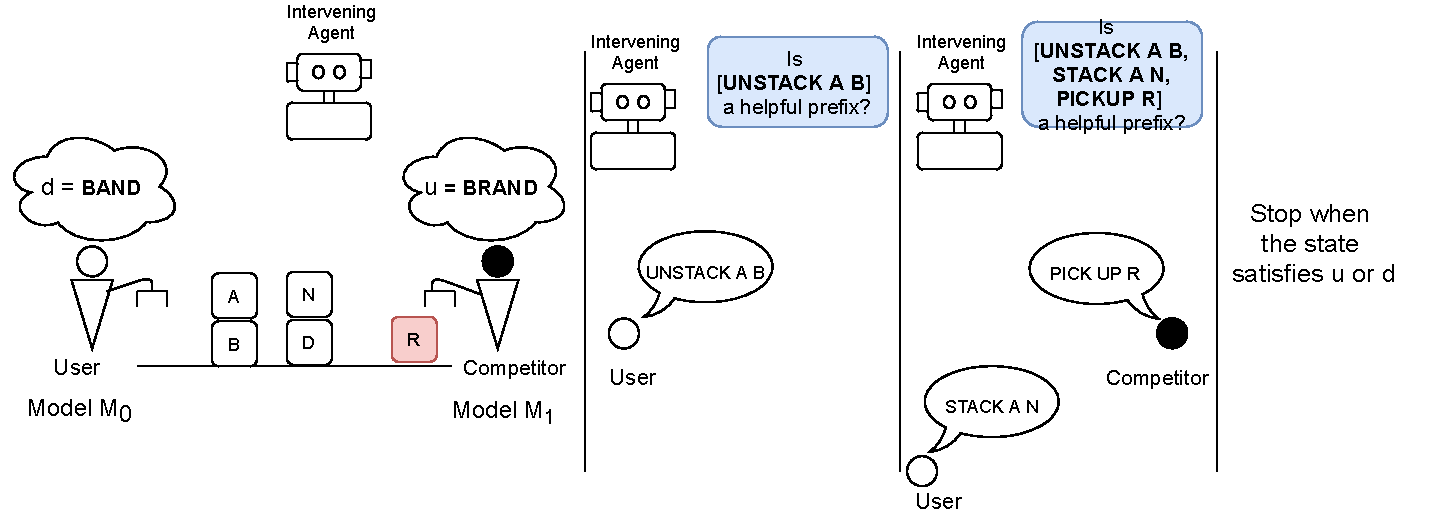
\includegraphics[width=1.1\columnwidth]{img/InterventionEpisode.pdf}
\end{figure}
\end{frame} %#3

\begin{frame}{Research Question: How to identify the salient characteristics for deciding to intervene?}
\begin{itemize}
	\item Compare solutions that contain undesirable moves and solutions that do not.

	\item Two sources of extracting characteristics:
	\begin{itemize}
		\item Intervention Graph
		\item Plans sampled from the plan space
	\end{itemize}
	
\end{itemize}

\end{frame}
	 %#4
\begin{frame}{Intervention by Unhelpful Plan Prefix Recognition}
Assumptions
\begin{itemize}
\item $\mathrm{d}$ is user's goal, $\mathrm{u}$ is the  undesirable goal
\item The observer has full observability of the actors' actions.
\item The observer knows about $\mathrm{d}$  and $\mathrm{u}$ and helps the user avoid $\mathrm{u}$ 
\item $\mathrm{u}$  is unknown to the user. 
\item $\mathrm{d}$  is unknown to the competitor (if present)
\item User can not recognize effects of competitor's actions. Some of user's own actions may have hidden effects
\item User follows a satisficing plan to reach $\mathrm{d}$, and may reach $\mathrm{u}$  unwittingly
\end{itemize}
The recognition problem \\
\textit{\textbf{Given the action history ($o_1, \ldots ,o_{i-1}$), and the proposed action $o_i$ must the prefix ($o_1, \ldots ,o_{i-1}$) be flagged to help the user avoid $\mathrm{u}$}?}
\end{frame}	 %#5
\begin{frame}{Unhelpful Plan Prefix Recognition - Intervention Graph}
\begin{itemize}
\item Produce the intervention graph from current state (root) to $\mathrm{u}=$(BRAND) and $\mathrm{d}=$(BAND)
\end{itemize}

\begin{figure}[tb]
        \centering{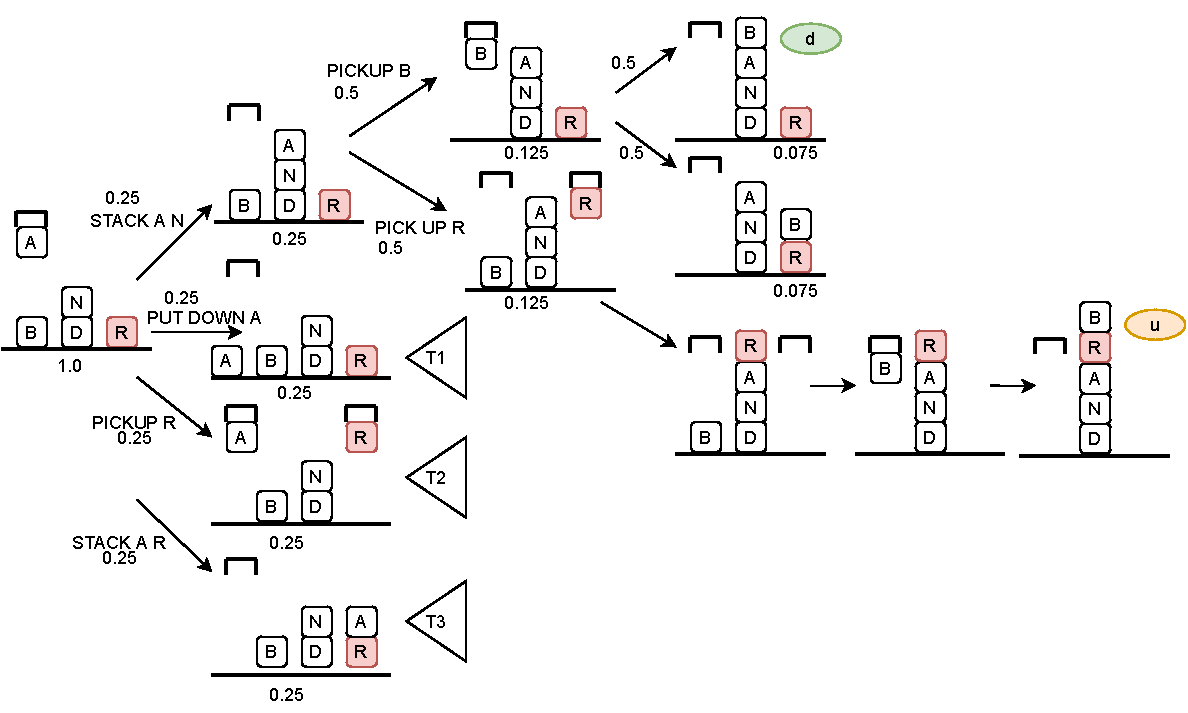
\includegraphics[width=\columnwidth]{img/BRAND_BAND.pdf}}
\end{figure} 

\end{frame}	 %#6
\begin{frame}

Compute features of critical actions (or sequences)
\begin{itemize}
\item \textbf{Risk} - Posterior probability of reaching $\mathrm{u}$, when the user is trying to reach $\mathrm{d}$
\item \textbf{Desirability} - Posterior probability of reaching $\mathrm{d}$, without passing $\mathrm{u}$
\item \textbf{Distance to} $\mathrm{d}$ - Mean number of edges between the root of the tree and $\mathrm{d}$, which doesn't pass through $\mathrm{u}$
\item \textbf{Distance to} $\mathrm{u}$ - Mean number of edges between the root of the tree and $\mathrm{u}$
\item \textbf{Active attack landmarks\%} - From the total number of predicates that must be true in any valid solution to the planning problem $\langle M,\mathrm{u}\rangle$, how many are true in the current state?
\end{itemize}

\end{frame}
	 %#7
\begin{frame}{Unhelpful Plan Prefix Recognition - Sampling the Plan Space}
\begin{itemize}
\item Instead of computing exact distances and probabilities compute an \textbf{estimated proximity to $\mathrm{d}$ and $\mathrm{u}$}
\item Use an automated planner to find two solution sets for $\langle M, \mathrm{d}\rangle$ and  $\langle M, \mathrm{u}\rangle$
\item Compute a \textit{reference plan} $= \lbrace observations + \pi^*\rbrace$, 
\begin{itemize}
\item $\pi^*$ - cost optimal plan from the current state to the goal for $\mathrm{d}$
\end{itemize}
\item Compute the ``distances'' between the \textit{reference plan} and the two solution sets


\begin{itemize}
\item Is the reference plan more similar to sampled $\mathrm{d}$ plans or $\mathrm{u}$ plans?
\item plan distance metrics: action set distance, causal link distance, state sequence distance, edit distance.
\end{itemize}

\end{itemize}

\end{frame}	 %#8
\begin{frame}{Learning to Intervene}
\begin{itemize}
\item Two feature sets:
\begin{itemize}
\item intervention graph metrics
\item distance metrics from the sampled plans
\end{itemize}
\item Use the feature sets to train classifiers to recognize unhelpful plan prefixes
\begin{itemize}
\item Naive Bayes, K-nearest neighbor, Decision tree, Logistic regression
\end{itemize}
\item Use the classifiers to recognize intervention in unseen problems
\end{itemize}

\end{frame} 	%#9
\begin{frame}{Classifier Performance}
Reporting F-score  $= \frac{TP}{TP + 1/2(FP+FN)}$ \\ Matthews Correlation Coefficient (MCC)
\begin{itemize}
\item Planning domains: BlocksWorld, EasyIPC, Ferry, Navigator, RushHour
\item Classifiers with Intervention Graph features
\begin{itemize}
\item High accuracy (F-Score, MCC $>$87\%) for all domains
\item Uniform high accuracy across different classifiers
\end{itemize}
\item Classifiers with plan distance metrics
\begin{itemize}
\item Accuracy varies for different types of classifiers for each domain
\item Blocksworld problems - \textbf{K-nearest neighbor}
\item EasyIPC/Navigator problems -\textbf{Naive Bayes}
\item Rush Hour problems -\textbf{Decision Tree, K-nearest neighbor}
\item Lowest accuracy for Ferry domain problems
\end{itemize}
\end{itemize}




\end{frame} 	%#10
\begin{frame}{Intervention with Existing Goal Recognition Algorithms}
\begin{itemize}
\item Use \textbf{plan recognition as planning} and \textbf{goal mirroring} to recognize likely goals given observations
\item If the likely goal is $\mathrm{u}$, then intervene
\item Results
\begin{itemize}
\item Reporting F-score and Matthews Correlation Coefficient (MCC) for benchmark planning domains (Blocks words, EasyIPC, Ferry)
\item Many false negatives/positives occur when the undesirable state is close to the desirable state in the state space.
\item Low accuracy in recognizing when intervention is required
\end{itemize}
\end{itemize}

\end{frame} 	%#11

\setbeamertemplate{section page}[questions]
\section{Questions?}

\end{document}